\chapter{Experiment Setup}\label{chp:6}

For our experimental setup, we will now generate data for both train and test sample under the conditions of covariate shift and show its effect on the model performance. We will also try to regularize the effect of covariate shift by importance weighting. In particular, we will use \emph{kernel density estimation} and \emph{self-attention mechanism} to estimate the weights.

\section{Covariate Shift in Linear Regression}

For our experiment and problem formulation, we focus on linear regression with a $10$-dimensional feature space and a scalar outcome. So, $\mathcal{X} = \mathbb{R}^{10}$ and $\mathcal{Y} = \mathbb{R}$, and our observations follow the model:

\begin{equation}
    y_i = f^*(x_i) + \epsilon_i, \quad f^*(x_i) = \langle \theta^*, x_i \rangle, \quad \epsilon_i \sim \mathcal{N}(0, \sigma^2)
    \label{eqn:6.1}
\end{equation}

\vspace{1em}
with $i = 1, \ldots, 1000$ and $\theta^* = \mathbf{1}^{10}$ (a vector of $1$). \\

The training set $\mathcal{S} = \{ (x_i, y_i) \}$ are independent and identically distributed (i.i.d) from $\mathbb{P}_{\text{train}} = \mathcal{N}(0, 1)$. We denote the design matrix by $\mathbf{X} \in \mathbb{R}^{1000 \times 10}$ and the vector of outputs by $\mathbf{Y} = (y_1, \ldots, y_{1000})^\top \in \mathbb{R}^{1000}$.\\

We also draw multiple test dataset $\mathcal{T}_{\mu} = \{ (\tilde{x}_t, \tilde{y}_t) \} \sim \mathcal{N}(\mu, 1)$ with $t = 1, \ldots, 1000$ and $\mu \in \{ 0, 0.2, 0.4, \ldots, 1.8, 2.0 \}$.\\

That means, we have $11$ test dataset, each with $\text{sample size} = 1000$ and \textcolor{blue}{\emph{mean shift}}. The multiple test dataset will help us understand the effect of varying mean shift in estimating the parameter $\hat{\theta} \in \mathbb{R}^{10}$ and the model performance.\\

\textbf{Note:} In practical situations, we do not know the underlying distributions of both train and test data. Here, for experimental purpose, we have generated the data following \emph{Gaussian distribution}, with test data having \emph{mean shift}.\\

\begin{figure}[h!]
    \centering
    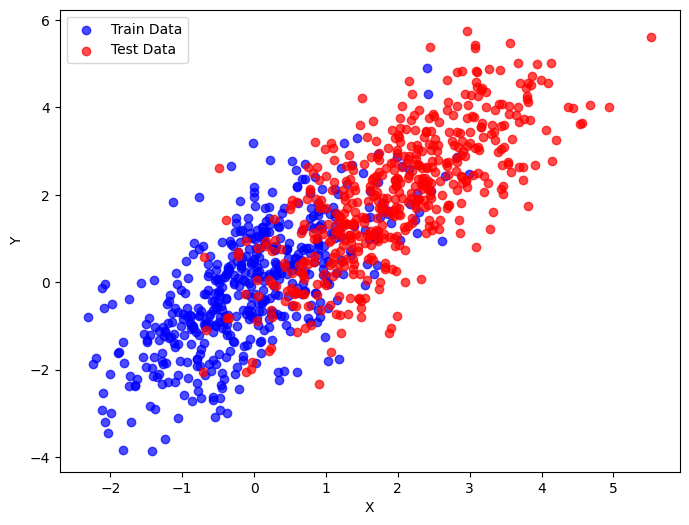
\includegraphics[width=0.7\textwidth]{images/Figure 0.png}
    \captionsetup{format=hang, singlelinecheck=false}
    \caption{Visual example of training data and test data drawn from Gaussian distribution with mean shift. Here, the training sample (in blue) are drawn from $\mathcal{N}(0,1)$ and the test sample (in red) are drawn from $\mathcal{N}(2, 1)$ each with a sample size of $500$ and the underlying relation: $y_i = x_i + \epsilon_i, \quad \epsilon_i \sim \mathcal{N}(0, 1), \quad i = 1, \ldots, 500$. This is just for visual example of how covariate shift effects and in our experiment, we are not working on this data.}
    \label{fig:0}
\end{figure}

\textbf{Measure of Performance}:\\

For our experiment, since we are focusing on linear regression, we have considered \textcolor{blue}{\emph{mean square error} (MSE)} as the \emph{loss function} to measure the error in predicting the outcome.\\

For an estimator $\hat{f}(x) = \langle \hat{\theta}, x \rangle$, the mean square error on a test sample $(\tilde{x}_i, \tilde{y}_i)$ is measured as:

\begin{equation}
    \text{MSE} = \frac{1}{n} \sum_{i=1}^n (\hat{f}(\tilde{x}_i) - \tilde{y}_i)^2 = \frac{1}{n} \sum_{i=1}^n \left( \langle \hat{\theta}, \tilde{x}_i \rangle - \tilde{y}_i \right)^2
    \label{eqn:6.2}
\end{equation}

i.e., the average squared difference between the true value and predicted value of the outcome, where $n$ is the number of samples in the test dataset.

\section{Effect of Mean Shift on MSE}

Now, we experiment how the mean shift $\mu$ affect the model performance in estimating the outcome using two most popular methods: \textcolor{blue}{\emph{Ordinary Least Square (OLS)}} and \textcolor{blue}{\emph{Gradient Descent}}.

\subsection{Ordinary Least Square (OLS) Estimator}

We briefly recall the definition of OLS for a \emph{design matrix} $\mathbf{X} \in \mathbb{R}^{n \times d}$ below.

\begin{definition}[Ordinary Least Squares]
When the design matrix $\mathbf{X}$ has full column rank, i.e., $\text{rank}(\mathbf{X}) = d$ meaning, the problem is \emph{overdetermined} and we have $n \geq d$ (more observations than feature dimensions), then the minimizer of the empirical risk (with least sqaure loss function)

\begin{equation}
    \mathcal{R}(\theta) = \frac{1}{n} \lVert \mathbf{Y} - \mathbf{X}\theta \rVert_2^2
    \label{eqn:6.3}
\end{equation}

is as below:

\begin{equation}
    \hat{\theta}_{\text{OLS}} := \argmin_{\theta \in \mathbb{R}} \mathcal{R}(\theta) = \argmin_{\theta \in \mathbb{R}} \frac{1}{n} \lVert \mathbf{Y} - \mathbf{X}\theta \rVert_2^2
    \label{eqn:6.4}
\end{equation}

and is called the \emph{Ordinary Least Squares} estimator.
\end{definition}

\begin{proposition}[Closed form solution of OLS]
If $\text{rank}(\mathbf{X}) = d$, we can show that $\hat{\theta}_{\text{OLS}}$ exists and is unique. It also attains a closed form solution \citep{aitken1936least, rao1945information}:

\begin{equation}
    \hat{\theta}_{\text{OLS}} = (\mathbf{X}^\top \mathbf{X})^{-1}\mathbf{X}^\top \mathbf{Y}
    \label{eqn:6.5}
\end{equation}
\end{proposition}

In our problem setting, we use this closed form solution to estimate the parameter $\theta$ and use them to predict the outcome for inputs $\tilde{x}$ from test dataset $\mathcal{T}_{\mu}$ for varying $\mu$. Finally, we measure our performance by calculating MSE and plot the resulting MSE against the corresponding mean shift ($\mu$).

\begin{figure}[h!]
    \centering
    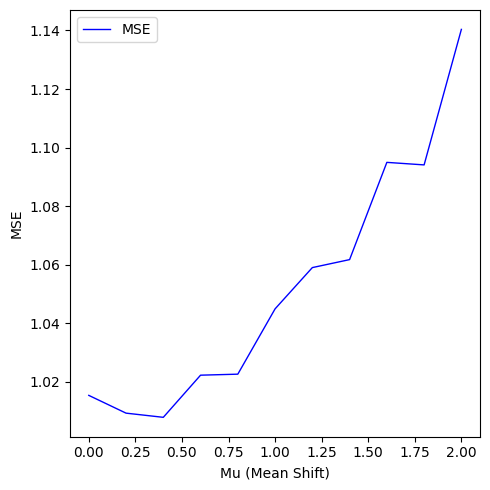
\includegraphics[width=0.5\textwidth]{images/Figure 1.png}
    \captionsetup{format=hang, singlelinecheck=false}
    \caption{Effect of varying mean shift on Mean Square Error (MSE) in Ordinary Least Square (OLS) estimator setup}
    \label{fig:1}
\end{figure}

Figure \ref{fig:1} illustrates the effect of covariate shift on model performance using ordinary least squares (OLS) estimator. As the mean shift ($\mu$) increases, the MSE also rises, indicating that the model's predictive accuracy deteriorates when the input distribution (test data) deviates from its training distribution. Initially, small shifts ($\mu < 0.5$) have a minor impact, but as $\mu$ grows, the error escalates more rapidly, suggesting a significant sensitivity to distributional changes. This behavior highlights the challenges posed by covariate shift.\\

\subsection{Gradient Descent Estimator}

Now, we will repeat the experiment with Gradient Descent with two different step size, $\gamma = 0.1$ and $\gamma=0.05$, to also observe the effect of step size ($\gamma$) on convergence rate. We recall the definition gradient descent before.

\begin{definition}[Gradient Descent]
The gradient descent is an iterative method where in each iteration, it moves towards the direction of steepest descent to move closer to the minima \citep{cauchy1847gradient}. It iterates with fixed step size $\gamma > 0$ and an initial parameter $\theta_0 \in \mathbb{R}^d$.\\

For a empirical risk with least-square loss function
\begin{equation}
    \mathcal{R}(\theta) = \frac{1}{n} \lVert \mathbf{Y} - \mathbf{X}\theta \rVert_2^2
    \label{eqn:6.6}
\end{equation}
the gradient is given by

\begin{equation}
    \begin{aligned}
        \nabla \hat{\mathcal{R}}(\theta) &= \frac{2}{n} \mathbf{X}^\top (\mathbf{X}\theta - \mathbf{Y})\\
        &= \frac{2}{n} \mathbf{X}^\top\mathbf{X}\theta - \frac{2}{n} \mathbf{X}^\top\mathbf{Y}
    \end{aligned}
    \label{eqn:6.7}
\end{equation}

and the estimated parameter $\hat{\theta}$ after $t+1$ iterations is given by
\begin{equation}
    \begin{aligned}
        \hat{\theta}_{t+1} &= \hat{\theta}_t - \gamma \nabla \hat{\mathcal{R}}(\hat{\theta}_t)\\
        &= (\mathbf{I}_d - 2 \frac{\gamma}{n}\mathbf{X}^\top \mathbf{X})\hat{\theta}_t + 2 \frac{\gamma}{n} \mathbf{X}^\top \mathbf{Y}
    \end{aligned}
    \label{eqn:6.8}
\end{equation}

\end{definition}

\begin{figure}[h!]
    \centering
    \begin{subfigure}{\textwidth}
        \centering
        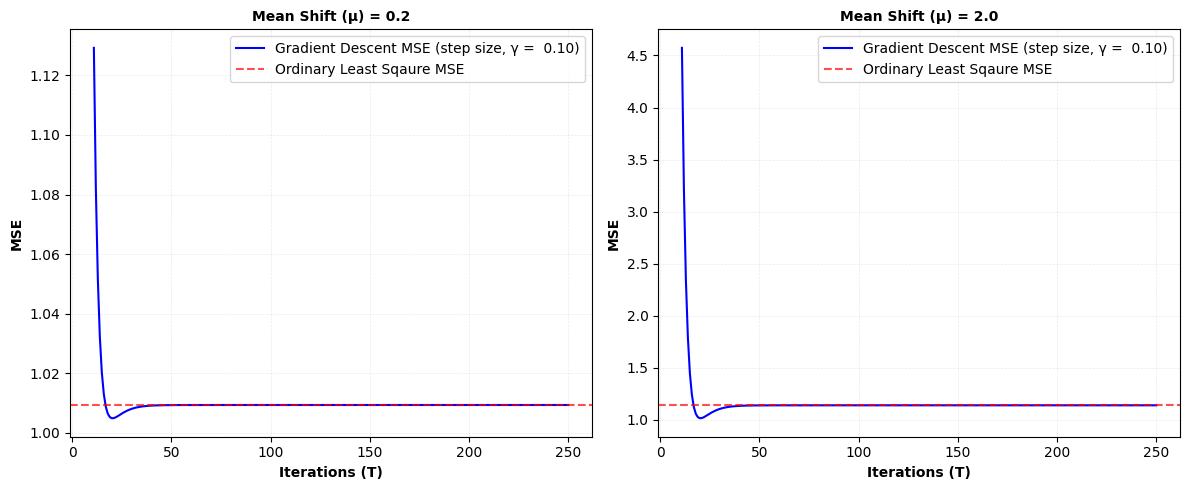
\includegraphics[width=\linewidth]{images/Figure 2a.png}
        \caption{Step size, $\gamma = 0.1$}
        \label{fig:2a}
    \end{subfigure}
    \hfill
    \begin{subfigure}{\textwidth}
        \centering
        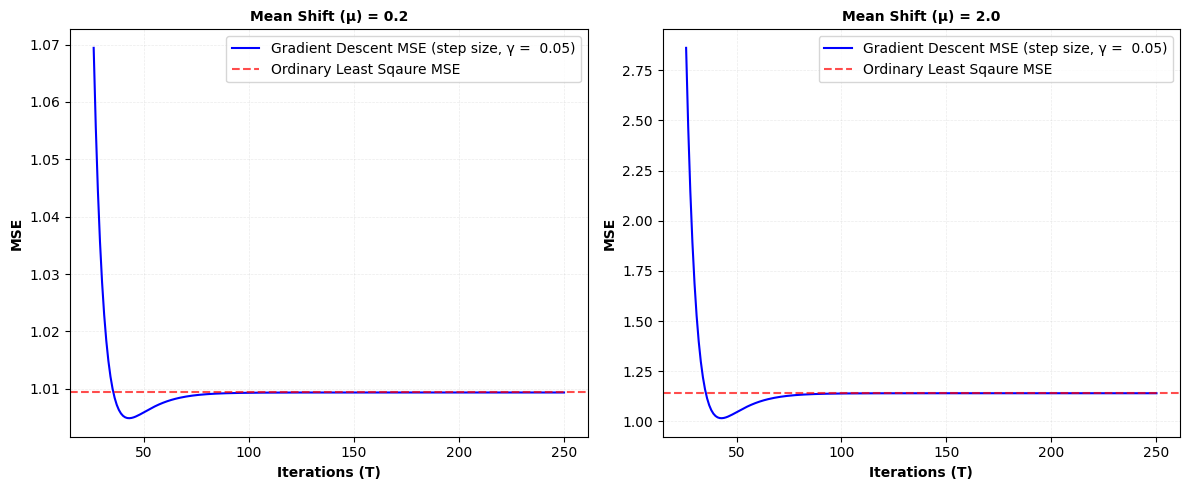
\includegraphics[width=\linewidth]{images/Figure 2b.png}
        \caption{Step size, $\gamma = 0.05$}
        \label{fig:2b}
    \end{subfigure}
    \captionsetup{format=hang, singlelinecheck=false}
    \caption{The image on left side plots the MSE against the increasing iterations for a mean shift, $\mu = 0.2$. The image on the right shows the same experiment for $\mu = 2.0$. We have chosen two extreme mean shift values to show the extreme effects. The experiment was carried out for two different step size, \textbf{(a)} $\gamma = 0.1$ and \textbf{(b)} $\gamma = 0.05$, to also observe the effect of step size ($\gamma$) on the convergence rate. \textbf{Note}: For better visualization purpose, the number of iterations on X-axis are truncated (initial few iterations are removed) in all plots to show the dip in curve prominently.}
    \label{fig:2}
\end{figure}

In our problem setting, we use $\theta_0 = \boldsymbol{0}^{10}$ (a vector of zero) and run the estimator for $250$ iterations, i.e., $\text{T}_{\text{max}} = 250$. We carry out the experiment using gradient descent for two different step sizes, $\gamma=0.1$ and $\gamma=0.05$.\\

Figure \ref{fig:2} illustrates the behavior of Mean Squared Error (MSE) using gradient descent method under different levels of covariate shift ($\mu = 0.2$ in left and $\mu = 2.0$ in right) and different step sizes, $\gamma=0.1$ in top and $\gamma=0.05$ in bottom. We observe that for gradient descent, the MSE initially starts at a high value and decreases rapidly as iterations increase, indicating convergence towards a minimum. However, for $\mu = 2.0$ (right), the initial MSE is significantly higher compared to $\mu = 0.2$ (left), suggesting that greater distribution shifts lead to higher initial errors. This behavior is observed for both step sizes and can be seen more precisely seen for all the mean shift ($\mu$) values in Figure \ref{fig:3}.\\

From Figure \ref{fig:2}, we also observe that irrespective of the choice of the step size ($\gamma$) and mean shift ($\mu$), the MSE dips below the OLS baseline before eventually converging towards it, implying that iterative optimization can momentarily outperform OLS but ultimately stabilizes around a similar error level. However, the convergence rate depends on the step size ($\gamma$), with higher $\gamma$ helps in converging faster. This can be observed in Figure \ref{fig:2a}, where the gradient descent with $\gamma=0.1$ converges to the OLS baseline in $\sim 40$ iterations, whereas it takes $\sim 80$ iterations with $\gamma=0.05$ (Figure \ref{fig:2b}).\\

Overall, the results from Figure \ref{fig:2} highlight the impact of covariate shift on learning dynamics, where larger shifts exacerbate the initial error but do not necessarily affect the final convergence behavior. Also, the choice of step size ($\gamma$) affects the convergence rate to a great extent. Since our main goal is to minimize the MSE as much as possible, so if we can select an \textcolor{blue}{\emph{optimal stopping time}} ($\text{T}_{\text{opt}}$), then gradient descent estimator will give us a better result than the baseline of ordinary least squares estimator.\\

By theory, the bias in expected excess risk decreases with the number of iterations, while the variance in expeced excess risk increases. At optimal stopping time ($\text{T}_{\text{opt}}$), we achieve a balance between these two (both becomes equal) and we found an upper bound of expected excess risk.

\begin{proposition}[Optimal Stopping Time and Upper Bound of Expected Excess Risk]
Choosing
\begin{equation}
    \text{T}_{\text{opt}} = \frac{\sqrt{n}\lVert \theta^* \rVert}{\gamma \sigma \sqrt{2 \text{ Trace}[\hat{\Sigma}]}},
    \label{eqn:6.9}
\end{equation}

the expected excess risk satisfies
\begin{equation}
    \mathbb{E}[\mathcal{R}(\hat{\theta}_{\text{T}_{\text{opt}}})] - \mathcal{R}^* \leq \frac{4\sigma \lVert \theta^* \rVert \text{ Trace}[\hat{\Sigma}]^{\frac{1}{2}}}{\sqrt{n}}
    \label{eqn:6.10}
\end{equation}

where $n$ is the sample size, $\sigma$ is the standard deviation in the noise $\epsilon$ and $\hat{\Sigma} = \frac{1}{n} \mathbf{X}^\top \mathbf{X}$ is the covariance matrix.
\end{proposition}

\begin{figure}[h!]
    \centering
    \begin{subfigure}{0.49\textwidth}
        \centering
        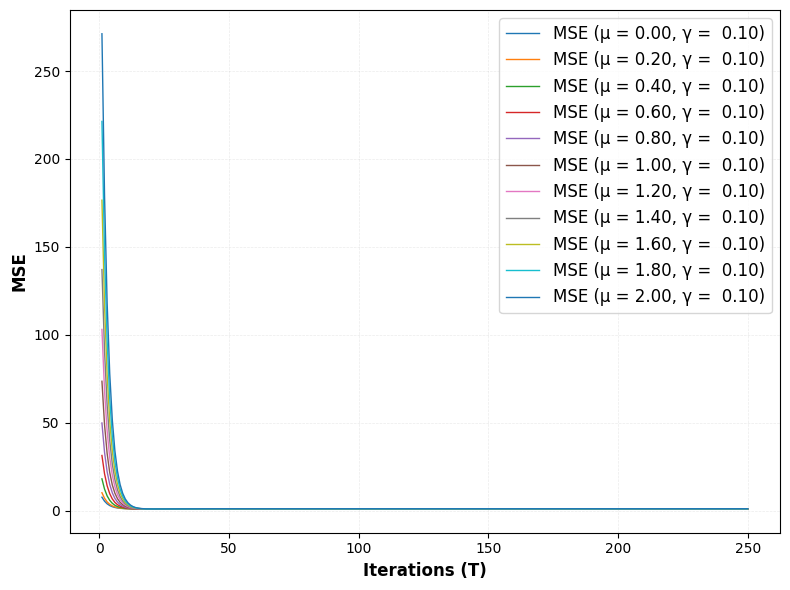
\includegraphics[width=\linewidth]{images/Figure 3a.png}
        \caption{Step size, $\gamma = 0.1$}
        \label{fig:3a}
    \end{subfigure}
    \hfill
    \begin{subfigure}{0.49\textwidth}
        \centering
        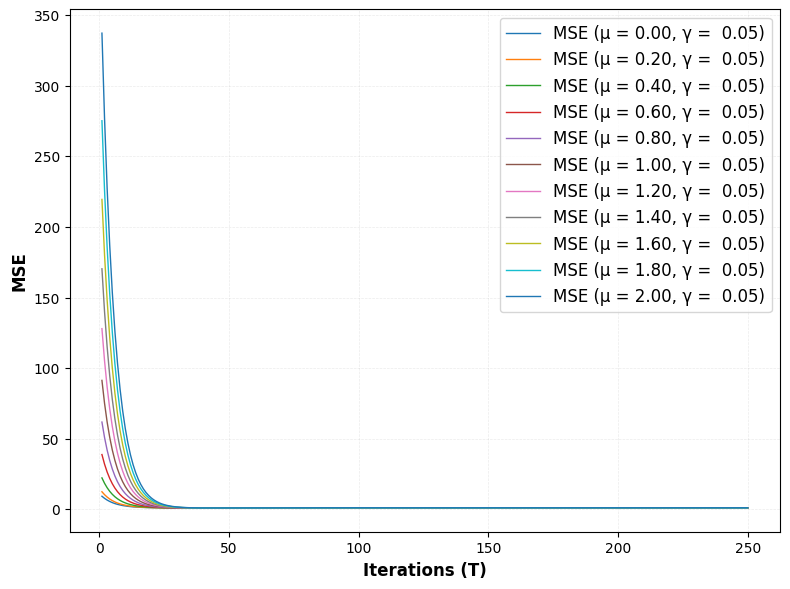
\includegraphics[width=\linewidth]{images/Figure 3b.png}
        \caption{Step size, $\gamma = 0.05$}
        \label{fig:3b}
    \end{subfigure}
    \captionsetup{format=hang, singlelinecheck=false}
    \caption{Initial value and rapid change in MSE with increasing iterations for multiple mean shifts, $\mu$. With a higher $\mu$, the initial value of MSE is greater compared to that with lower $\mu$. Also, with \textbf{(a)} higher step size ($\gamma = 0.1$), gradient descent converges much faster than gradient descent with \textbf{(b)} lower step size ($\gamma = 0.05$).}
    \label{fig:3}
\end{figure}

Figure \ref{fig:4} shows, more prominently using a heatmap, what we already observed before. A lower value of $\mu$ results in a much greater MSE initially as compared to the MSE for a higher $\mu$. As one can expect, for higher mean shift ($\mu$), it also takes longer iterations for the gradient descent to converge and reach minimum. The convergence rate also depends on the step size ($\gamma$): a higher step size ($\gamma = 0.1$) (Figure \ref{fig:4a}) achieves faster convergence than a lower step size ($\gamma = 0.05$) (Figure \ref{fig:4b}).\\

\begin{figure}[h!]
    \centering
    \begin{subfigure}{0.49\textwidth}
        \centering
        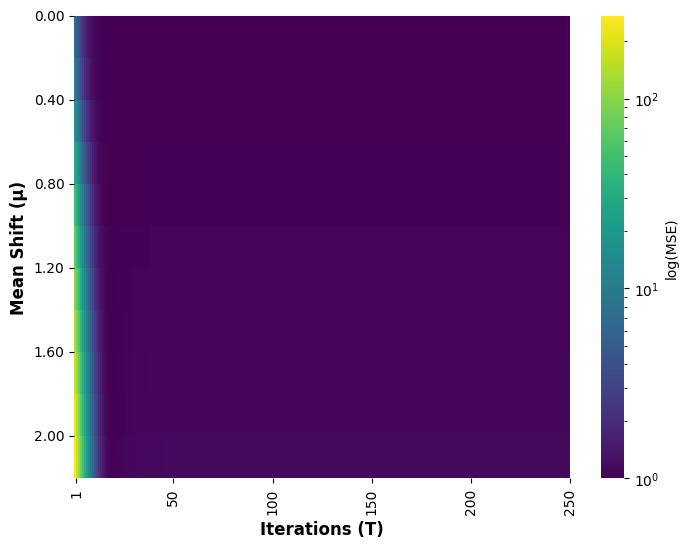
\includegraphics[width=\linewidth]{images/Figure 4a.png}
        \caption{Step size, $\gamma = 0.1$}
        \label{fig:4a}
    \end{subfigure}
    \hfill
    \begin{subfigure}{0.49\textwidth}
        \centering
        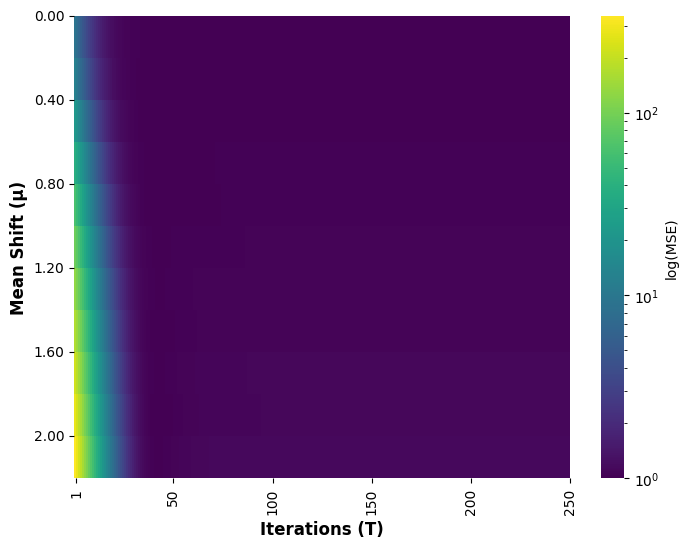
\includegraphics[width=\linewidth]{images/Figure 4b.png}
        \caption{Step size, $\gamma = 0.05$}
        \label{fig:4b}
    \end{subfigure}
    \captionsetup{format=hang, singlelinecheck=false}
    \caption{Heatmap of MSE to compare mean shift ($\mu$), iterations ($\text{T}$) and MSE in a single plot. Higher mean shift results in greater MSE initially and naturally it takes longer iterations for the gradient descent to minimize the MSE. Results are illustrated with \textbf{(a)} $\gamma = 0.1$ and \textbf{(b)} $\gamma = 0.05$. The logarithm of MSE is taken in the color bar for better scaling.}
    \label{fig:4}
\end{figure}


\begin{figure}[h!]
    \centering
    \begin{subfigure}{0.6\textwidth}
        \centering
        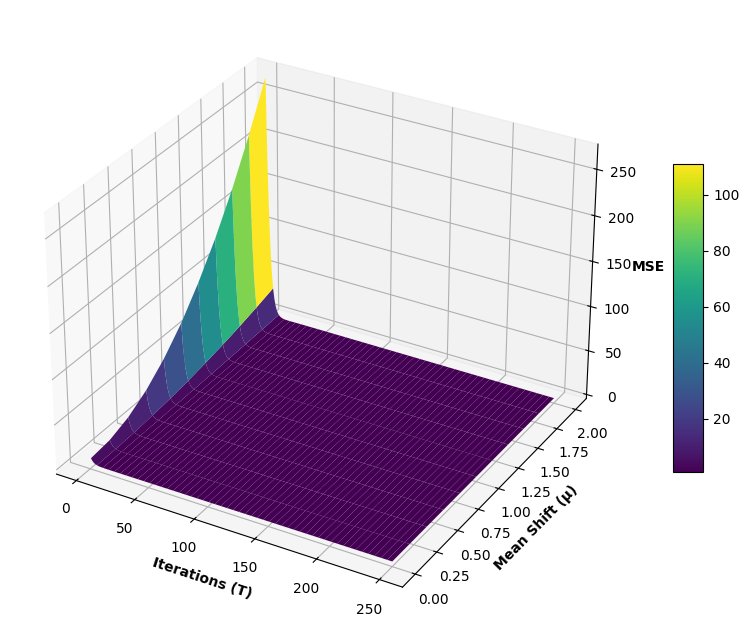
\includegraphics[width=\linewidth]{images/Figure 8a.png}
        \caption{Step size, $\gamma = 0.1$}
        \label{fig:5a}
    \end{subfigure}
    \hfill
    \begin{subfigure}{0.6\textwidth}
        \centering
        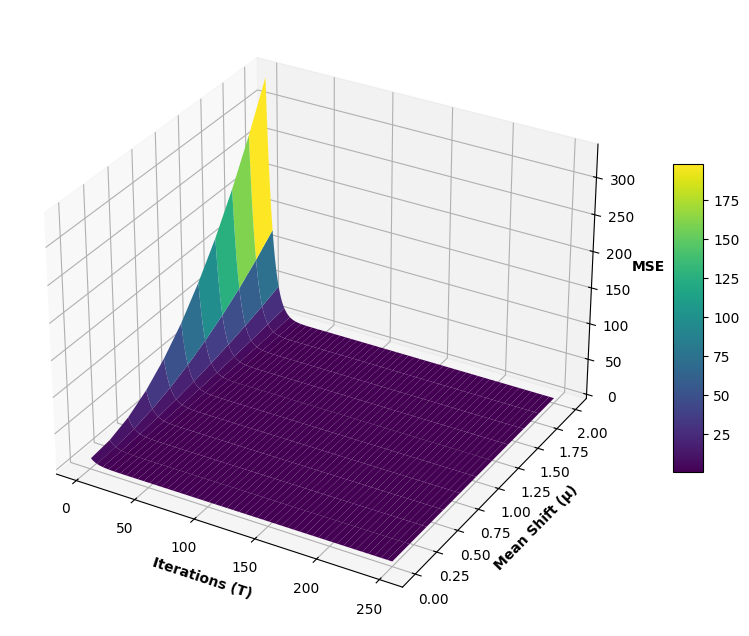
\includegraphics[width=\linewidth]{images/Figure 8b.png}
        \caption{Step size, $\gamma = 0.05$}
        \label{fig:5b}
    \end{subfigure}
    \captionsetup{format=hang, singlelinecheck=false}
    \caption{$3$-dimensional surface plot of interplay among mean shift ($\mu$), iteration count ($\text{T}$) and the respective mean square error (MSE) value in gradient descent method. The experiment was run using both \textbf{(a)} step size, $\gamma = 0.1$ and \textbf{(b)} step size, $\gamma = 0.05$.}
    \label{fig:5}
\end{figure}

The 3D plot in Figure \ref{fig:5} again visualizes the relationship between MSE (Mean Squared Error), iteration count in gradient descent ($\text{T}$), and mean shift ($\mu$) using two different step sizes, $\gamma = 0.1$ and $\gamma = 0.05$. Both plot shows that for small values of $\mu$, the MSE remains relatively low and stable as iterations increase. However, for larger values of $\mu$, the initial MSE is significantly higher, indicating a stronger negative impact of distribution shift on model performance. As iterations progress, the MSE decreases and stabilizes, suggesting convergence. The steep rise at the beginning for large $\mu$ values highlights the sensitivity of the model to distributional changes.\\


\begin{figure}[h]
    \centering
    \begin{subfigure}{0.48\textwidth}
        \centering
        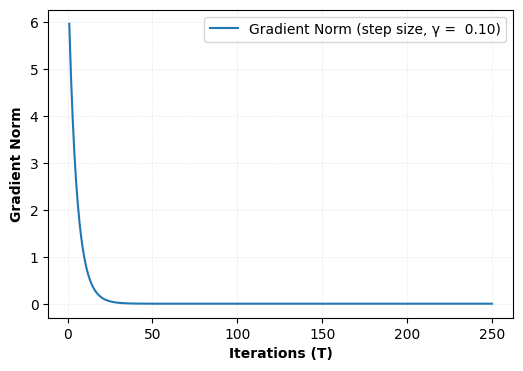
\includegraphics[width=\linewidth]{images/Figure 5a.png}
        \caption{Step size, $\gamma = 0.1$}
        \label{fig:6a}
    \end{subfigure}
    \hfill
    \begin{subfigure}{0.48\textwidth}
        \centering
        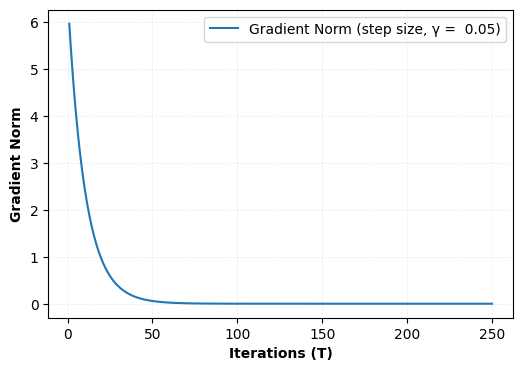
\includegraphics[width=\linewidth]{images/Figure 5b.png}
        \caption{Step size, $\gamma = 0.05$}
        \label{fig:6b}
    \end{subfigure}
    \hfill
    \begin{subfigure}{0.48\textwidth}
        \centering
        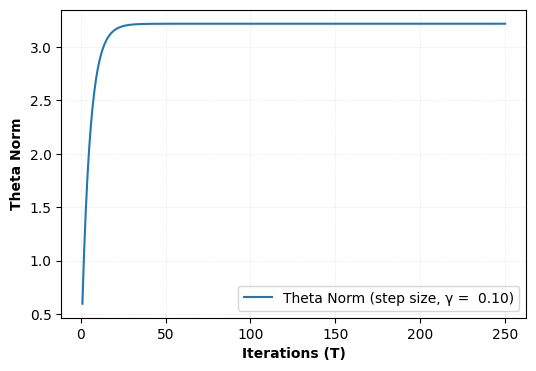
\includegraphics[width=\linewidth]{images/Figure 6a.png}
        \caption{Step size, $\gamma = 0.1$}
        \label{fig:6c}
    \end{subfigure}
    \hfill
    \begin{subfigure}{0.48\textwidth}
        \centering
        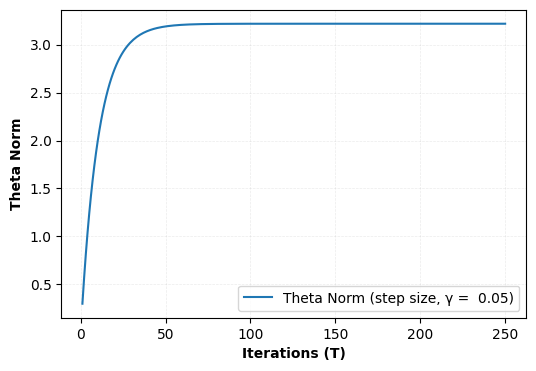
\includegraphics[width=\linewidth]{images/Figure 6b.png}
        \caption{Step size, $\gamma = 0.05$}
        \label{fig:6d}
    \end{subfigure}
    \captionsetup{format=hang, singlelinecheck=false}
    \caption{Illustration of how \textbf{(a)}, \textbf{(b)} the gradient norm $\lVert \nabla \hat{\mathcal{R}}(\theta) \rVert$ and \textbf{(c)}, \textbf{(d)} parameter norm $\lVert \hat{\theta}^{\text{GD}} \rVert$ change across iterations during the training using gradient descent method.}
    \label{fig:6}
\end{figure}

Figure \ref{fig:6} shows how the gradient norm $\lVert \nabla \hat{\mathcal{R}}(\theta) \rVert$ (Figure \ref{fig:6a} and Figure \ref{fig:6b}) and parameter norm $\lVert \hat{\theta}^{\text{GD}} \rVert$ (Figure \ref{fig:6c} and Figure \ref{fig:6d}) change during the gradient descent iterations. Since we learn the parameter only from the training sample $\mathcal{S} \sim \mathcal{N}(0, 1)$, this does not depend on the mean shift ($\mu$).\\

As we observe in Figure \ref{fig:6a} and \ref{fig:6b}, $\lVert \nabla \hat{\mathcal{R}}(\theta) \rVert$ initially starts with very high value and then with increasing iterations it steeply reduces, finally converging to $0$ in $\sim 30$ iterations for $\gamma=0.1$ and in $\sim 60$ iterations for $\gamma=0.05$. This is because the gradient norm measures how large the gradient is at a given point. A large gradient norm means the function is steep, and updates will be large, whereas, a small gradient norm means the function is flat, and updates will be small. At the beginning, the gradient norm is high because the parameters are far from the optimal values. As iterations progress, the optimizer moves downhill in the loss landscape, reducing both the loss and the gradient norm. Closer to the minimum, the gradient norm approaches zero because the function is nearly flat (stationary point).\\

The same logic explains the observations in Figure \ref{fig:6c} and \ref{fig:6d}. Initially, 
$\lVert \hat{\theta}^{\text{GD}} \rVert$, representing the norm (magnitude) of the parameter vector $\theta$, starts near zero. It rapidly increases within the first few iterations. The rate of increase slows down, and 
finally it plateaus at a final value around $\approx 3.2$ in $\sim 30$ and $\sim 60$ iterations respectively for $\gamma=0.1$ and $\gamma=0.05$. We recall that the parameters are updated in iterations by taking a step towards the gradient direction: $\hat{\theta}_{t+1} = \hat{\theta}_t - \gamma \nabla \hat{\mathcal{R}}(\hat{\theta}_t)$. At the beginning, gradient updates are large because the model parameters are far from optimal. As the optimizer updates $\theta$ through iterations, it moves towards an optimal region, causing the norm to increase. Eventually, closer to the minimum, the gradient approaches zero, meaning the parameters stabilize, and further updates are minimal.\\

Moreover, we also observe how it takes significantly less number of iterations for both the norms to reach its optimal value by increasing the step size from $\gamma=0.05$ to $\gamma=0.1$.



\subsection{Comparison between OLS and GD estimator (Effect of Mean Shift)}

We finally compare the performance from both ordinary least squares and gradient descent estimator (with different step sizes) for varying $\mu$ to observe the affect of mean shift on their performance.\\

\begin{figure}[h!]
    \centering
    \begin{subfigure}{\textwidth}
        \centering
        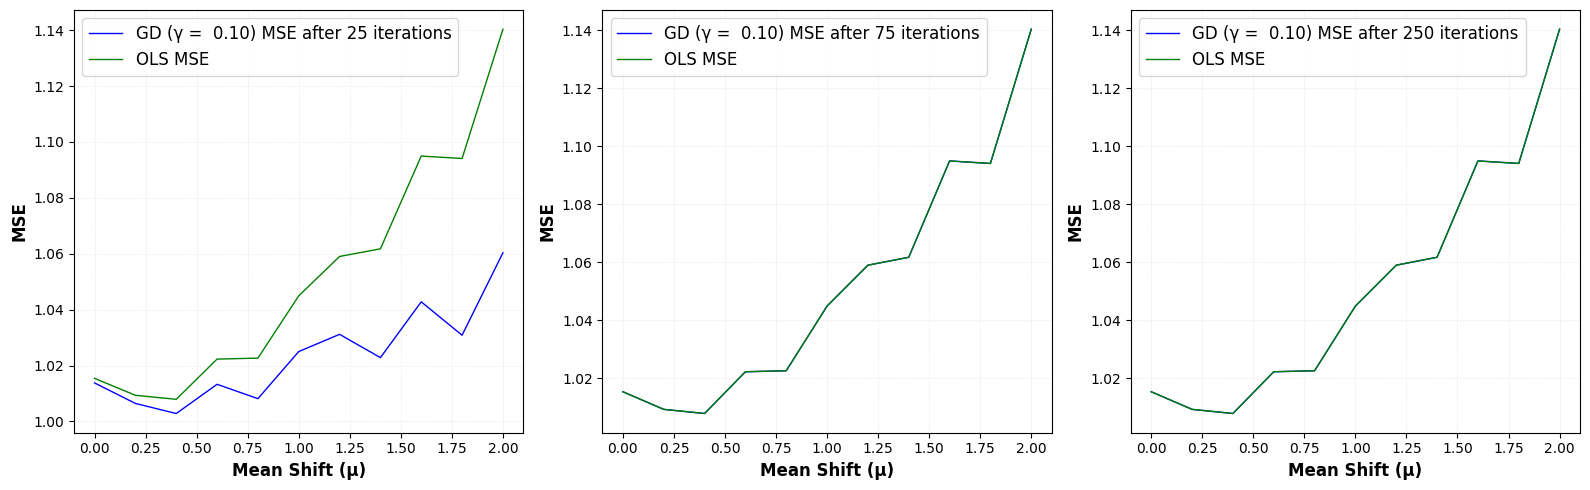
\includegraphics[width=\linewidth]{images/Figure 7a.png}
        \caption{Step size, $\gamma = 0.1$}
        \label{fig:7a}
    \end{subfigure}
    \hfill
    \begin{subfigure}{\textwidth}
        \centering
        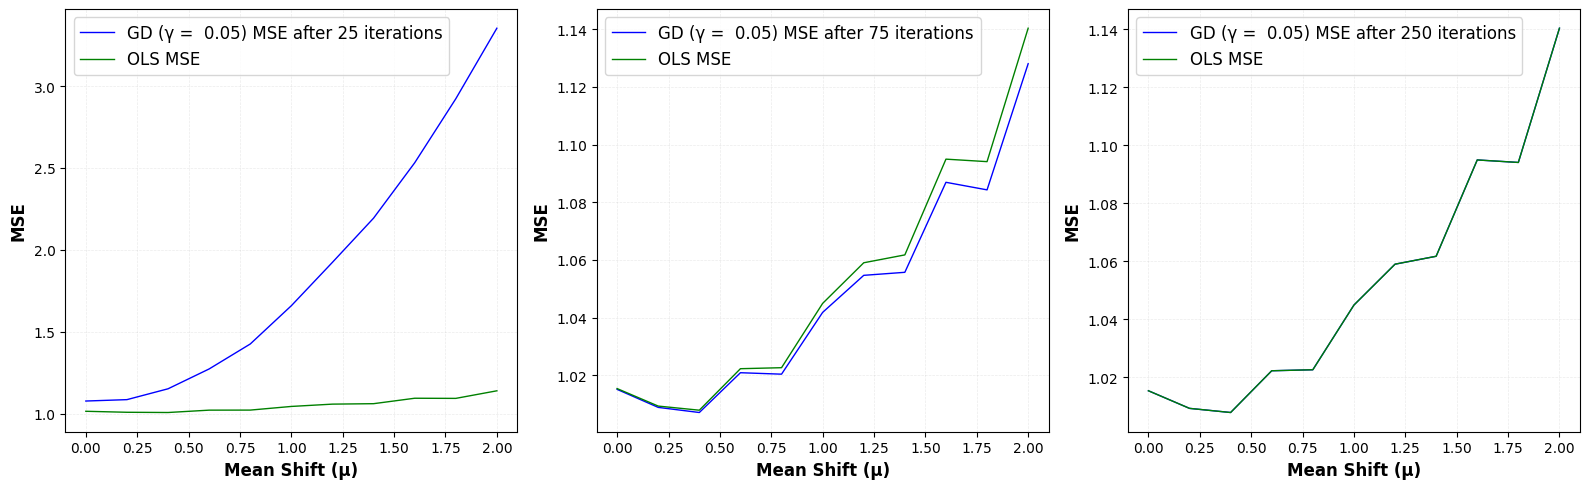
\includegraphics[width=\linewidth]{images/Figure 7b.png}
        \caption{Step size, $\gamma = 0.05$}
        \label{fig:7b}
    \end{subfigure}
    \captionsetup{format=hang, singlelinecheck=false}
    \caption{Mean Squared Error (MSE) of Gradient Descent (GD) and Ordinary Least Squares (OLS) as a function of Mean Shift ($\mu$), for different numbers of iterations ($\text{T}$): (I) results at $\text{T}=25$, (II) results at $\text{T} = 75$ and (III) results at $\text{T} = 250$. This is to observe the results during the beginning, after a few iterations and at the very end of the total iterations in gradient descent. The experiment is done twice for different step sizes: \textbf{(a)} $\gamma=0.1$ and \textbf{(b)} $\gamma=0.05$}
    \label{fig:7}
\end{figure}

The three-panel plot in Figure \ref{fig:7} plots the Mean Squared Error (MSE) obtained in Gradient Descent (GD) and Ordinary Least Squares (OLS) for different mean shift ($\mu$). We have plotted the result for three different iteration count ($\text{T}$): the leftmost plot corresponds to $\text{T}=25$, the middle plot to $\text{T} = 75$, and the rightmost plot to $\text{T}=250$. The three plots above (Figure \ref{fig:7a}) represents gradient descent with step size, $\gamma = 0.1$ while the three plots below (Figure \ref{fig:7b}) represents gradient descent with step size, $\gamma = 0.05$.\\

We can observe that initially at $\text{T}=25$, the GD MSE (blue) is significantly higher than the OLS MSE (green) for both values of $\gamma$, indicating that GD has not fully converged. Moreover, lower step size produces a smoother curve as the updates in each iterations are slower. As iterations increase to $\text{T} = 75$, the GD MSE with $\gamma = 0.05$ aligns almost closely with the OLS MSE, while the GD MSE with $\gamma = 0.1$ has already converged with the OLS MSE, suggesting better convergence. At $\text{T}=250$, GD and OLS produce identical errors, confirming that GD has converged to the optimal solution.\\

Additionally, across all plots, the MSE increases with $\mu$ for both gradient descent and OLS, indicating that a larger mean shift negatively impacts predictive accuracy. This behavior is expected since shifting the mean introduces distributional changes, making model estimation less effective. Overall, the results highlight that GD requires sufficient iterations to achieve optimal performance but can eventually approximate OLS solutions when properly tuned. The number of iterations also depends on the step size, $\gamma$.

\section{Regularizing Covariate Shift}

In the following section, we will try to regularize the affect mean shift ($\mu$) using importance weighting. We will use two different methods to estimate the weights: \emph{kernel density estimation} and \emph{self-attention mechanism}.

\subsection{Importance Weighting using Kernel Density Estimation}

As we recall from section \ref{imp-weight}, if $p_{\text{train}}(X)$ and $p_{\text{test}}(X)$ are the probability density functions of the input distribution $\mathbb{P}_{\text{train}}(X)$ and $\mathbb{P}_{\text{test}}(X)$ respectively, then the \textcolor{blue}{\emph{importance weights}} can be estimated as the ratio of test and training input densities at training input points:

\begin{equation}
    \omega(x_i) = \frac{p_{\text{test}}(x_i)}{p_{\text{train}}(x_i)}
    \label{eqn:6.11}
\end{equation}

$\mathbb{P}_{\text{train}}(X)$ and $\mathbb{P}_{\text{test}}(X)$ are also called \emph{source distribution} and \emph{target distribution} respectively.\\

In practical situations, we do not know which distribution is the training and test samples are drawn from. So the underlying probability density functions are also unknown. In such cases, we try to estimate the probability density function (PDF). One such method is \textcolor{blue}{\emph{Kernel Density Estimation}}.\\

\vspace{2em}
\textbf{Importance Weighted variant: Ordinary Least Square (OLS)}\\

We use the closed form solution in equation \ref{eqn:3.10} to compute the MSE in importance weighted setting using OLS estimator. For our experimental purpose, we have used \emph{Gaussian Kernel} to estimate the densities, as mentioned in equation \ref{eqn:3.5}.\\

Figure \ref{fig:9} compares the MSE calculated through standard OLS estimator (unweighted) and its importance weighted variant across varying mean shift ($\mu$). The comparison is done at different bandwidth level.\\

We recall that bandwidth controls the smoothness of the kernel density estimate. A smaller bandwidth produces a more detailed (possibly noisy) density estimate while a larger bandwidth produces a smoother density estimate, which might oversmooth the data and lose details. This behavior can be observed in Figure \ref{fig:9}. While with a smaller bandwidth, the estimated density is noisy (irregular), making the difference between MSE calculated for unweighted and weighted OLS greater and erratic. With a higher bandwidth ($h > 2.0$), the density becomes smoother and stable, hence the MSE of weighted OLS approaches towards the MSE of unweighted OLS. There might be even some loss of details contributing to this convergence.\\

We also observe in Figure \ref{fig:9} that the difference between MSE calculated for unweighted and weighted OLS increases with higher mean shift ($\mu$). This behavior is expected since shifting the mean introduces distributional changes, which results in the greater difference in respective MSE values.

\begin{figure}[h!]
    \centering
    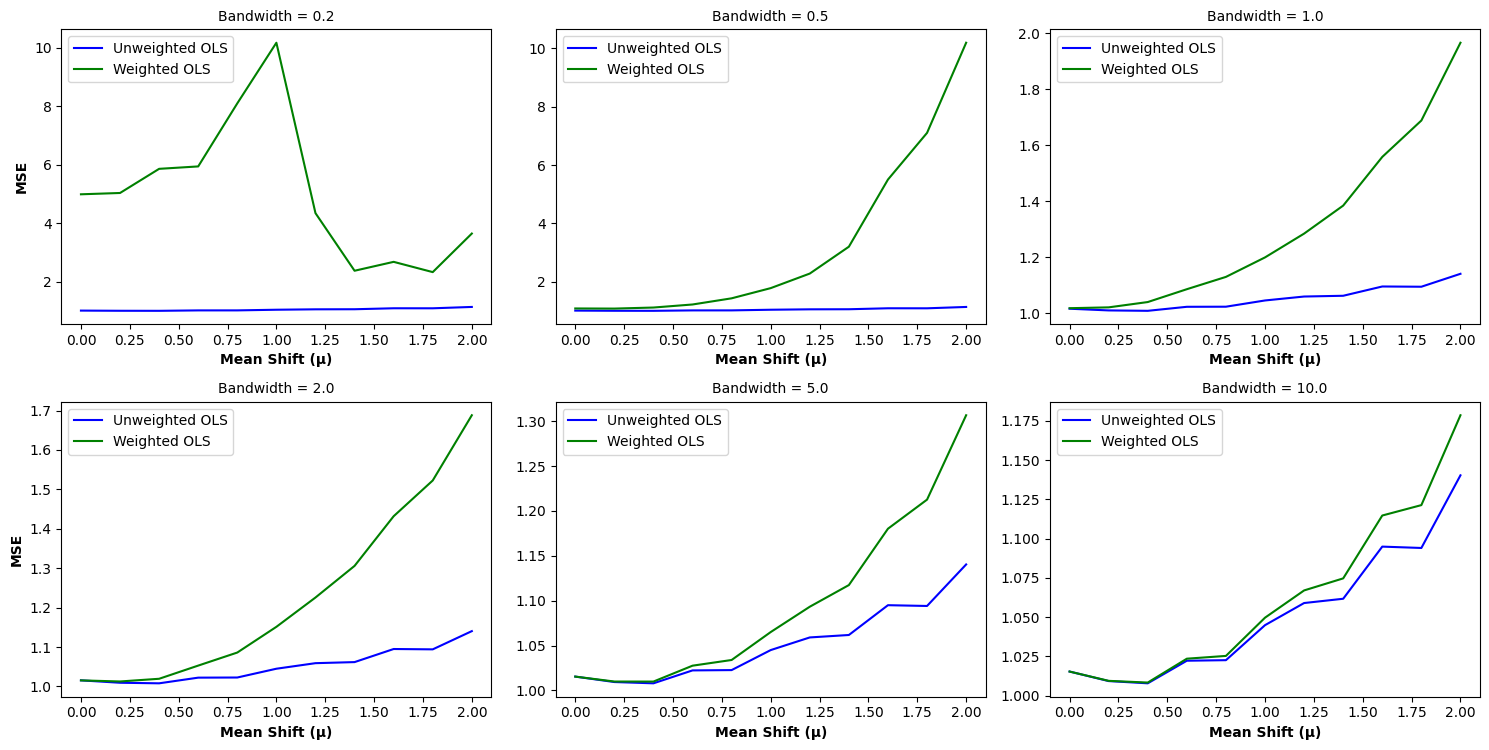
\includegraphics[width=\textwidth]{images/Figure 9.png}
    \captionsetup{format=hang, singlelinecheck=false}
    \caption{Effect of Importance Weighting (Kernel Density Estimation) with different bandwidth on MSE in Mean Shift setup. The MSE is calculated for both standard ordinary least square (unweighted) and importance weighted least square estimator at different bandwidth: (a) $h = 0.2$, (b) $h = 0.5$, (c) $h = 1.0$, (d) $h = 2.0$, (e) $h = 5.0$, (f) $h = 10.0$.}
    \label{fig:9}
\end{figure}

But even with the importance weighting, the regularization effect is not prominent since the MSE for weighted variant of OLS is consistently higher than that of unweighted variant (Figure \ref{fig:9}). This can have multiple reasons. To investigate further whether the sample size plays any role in the effect of mean shift on MSE, we plot the MSE for different sample sizes. At this moment, we \textbf{fix the mean shift} at $\mu = 1.0$ and use \textbf{fixed bandwidth} $=0.5$ (using \emph{Silverman's rule of thumb}: $h = 1.06 \times \sigma \times n^{-\frac{1}{5}}$, where $\sigma$ is the standard deviation of the data and $n$ is the sample size).

\begin{figure}[h!]
    \centering
    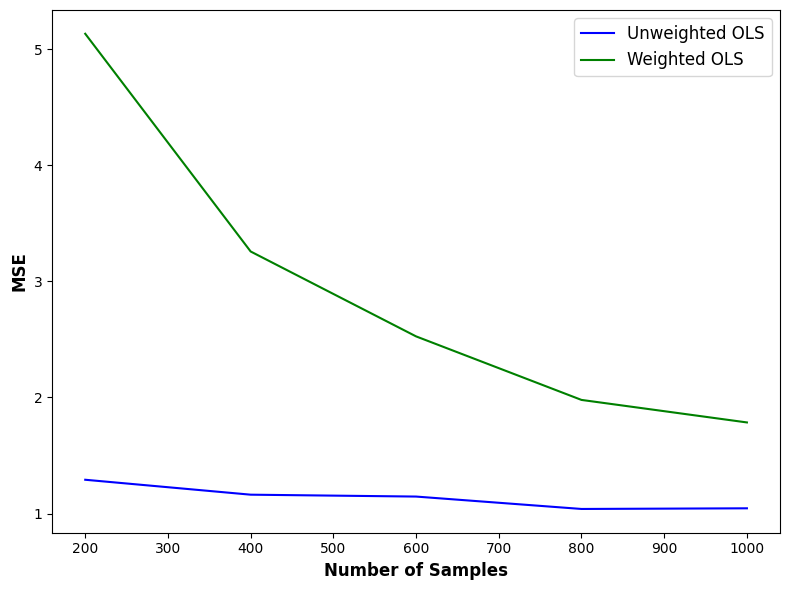
\includegraphics[width=0.7\textwidth]{images/Figure 10.png}
    \captionsetup{format=hang, singlelinecheck=false}
    \caption{Effect of sample size on mean shift regularization using importance weighting. The comparison is done between unweighted ordinary least square and importance weighted ordinary least square method at fixed mean shift ($\mu = 1.0$) and fixed bandwidth ($h=0.5$).}
    \label{fig:10}
\end{figure}

As we observe in Figure \ref{fig:10}, the sample size indeed plays a role. With higher sample sizes, the MSE calculated with weighted variant of OLS decreases rapidly and approaches the MSE of unweighted OLS. Due to limitation of computational resources, we couldn't experiment with any higher sample size, however this behavior is consistent with what we already discussed in section \ref{IWERM}, equation \ref{eqn:4.20}:
$$\lim_{n \to \infty} (\hat{\theta}_{\text{IWOLS}}) = \theta^*$$

Further investigation is required to investigate whether any other factors other than sample size plays a crucial role in regularizing the effect of mean shift by importance weighting.

\vspace{2em}
\textbf{Importance Weighted variant: Gradient Descent (GD)}\\

Similar to OLS, We use \ref{eqn:3.11} and \ref{eqn:3.12} to compute the MSE in importance weighted setting using OLS estimator. At this moment, we fix the mean shift at $\mu = 1.0$ and step size, $\gamma = 0.1$, bandwidth $= 0.5$ and increase the iteration count, $\text{T to } 5000$.\\

\begin{figure}[h!]
    \centering
    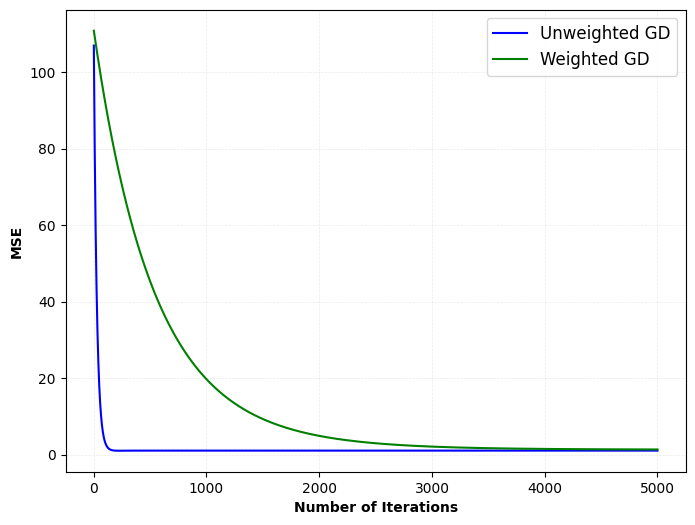
\includegraphics[width=0.6\textwidth]{images/Figure 11.png}
    \captionsetup{format=hang, singlelinecheck=false}
    \caption{Effect of importance weighting in mean shift regularization: Comparing MSE with unweighted and weighted variants of gradient descent, computed with step size, $\gamma = 0.1$ and iteration count, $\text{T} = 5000$. The experiment is done with fixed mean shift, $\mu = 1.0$ and bandwidth $= 0.5$.}
    \label{fig:11}
\end{figure}

Figure \ref{fig:11} shows the effect of importance weighting in regularizing the effect of mean shift by comparing the MSE calculated with both unweighted and weighted variants of gradient descent method. We observe here that with increasing iterations, the MSE calculated with weighted version of gradient descent is reducing steadily and approaching towards the MSE calculated with unweighted version of gradient descent, finally converging in $\sim 4000$ iterations. It was observed during the experiment that step size ($\gamma$) plays a crucial role, reducing it will take significantly more number of iterations to converge.\\

Once again, we try to investigate whether sample size plays any role in regularizing effect. As we observe in Figure \ref{fig:12}, increasing the sample size helps in regularizing the effect of mean shift. Keeping the number of iterations fixed at $\text{T} = 5000$, we can see that as sample size increases, performance of weighted gradient descent steadily approaches towards that of unweighted version and \emph{almost} converges with $1000$ sample sizes. Working with further sample size will require more computational resources.

\begin{figure}[h!]
    \centering
    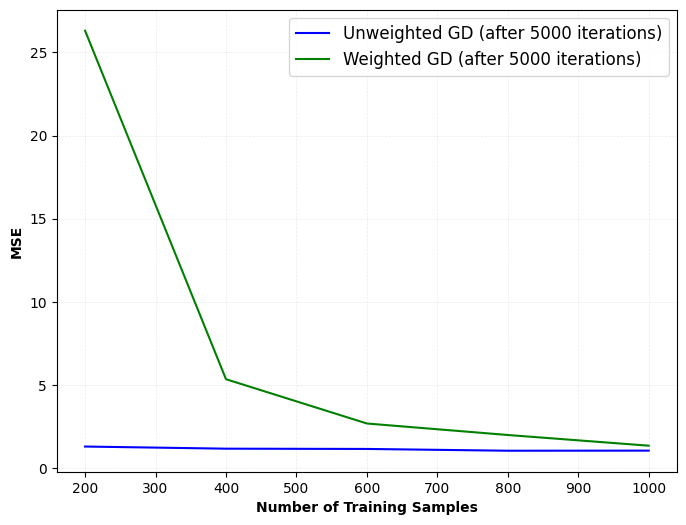
\includegraphics[width=0.5\textwidth]{images/Figure 12.png}
    \captionsetup{format=hang, singlelinecheck=false}
    \caption{Effect of sample size on regularizing mean shift by importance weighted gradient descent with $\text{T} = 5000$ iterations, step size, $\gamma = 0.1$ and sample size $=1000$.}
    \label{fig:12}
\end{figure}

In Figure \ref{fig:13}, we compare the performance of weighted OLS and weighted GD estimator, with a step size, $\gamma = 0.1$. We can observe here that unlike in the unweighted setup (Figure \ref{fig:2}), in the weighted setup, the gradient descent converges to OLS very steadily even with the same step size. It takes significantly higher number of iterations to converge to OLS compared to unweighted setup.\\

\begin{figure}[h!]
    \centering
    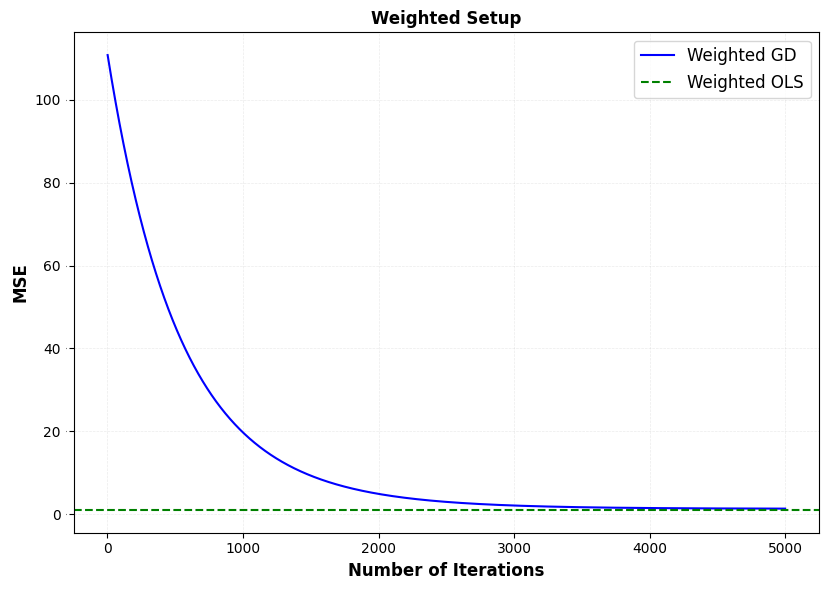
\includegraphics[width=0.6\textwidth]{images/Figure 13.png}
    \captionsetup{format=hang, singlelinecheck=false}
    \caption{Comparison of weighted OLS and weighted GD (step size, $\gamma = 0.1$) performance across iterations for fixed mean shift, $\mu = 1.0$.}
    \label{fig:13}
\end{figure}

One of the reason for this erratic behavior is of course is the sample size, as we have already established. Figure \ref{fig:14} shows the effect of sample size on regularizing mean shift by importance weighted variants of both OLS and gradient descent. Here we again compare the performance of gradient descent with that of OLS, in both weighted and unweighted setup, but in terms of sample size while keeping the iteration count fixed at $\text{T} = 5000$. This is in contrast to Figure \ref{fig:13}, where we had kept the sample size constant at $n = 1000$ and measured the performance against varying iteration count, $\text{T}$, in weighted setup.

\begin{figure}[h!]
    \centering
    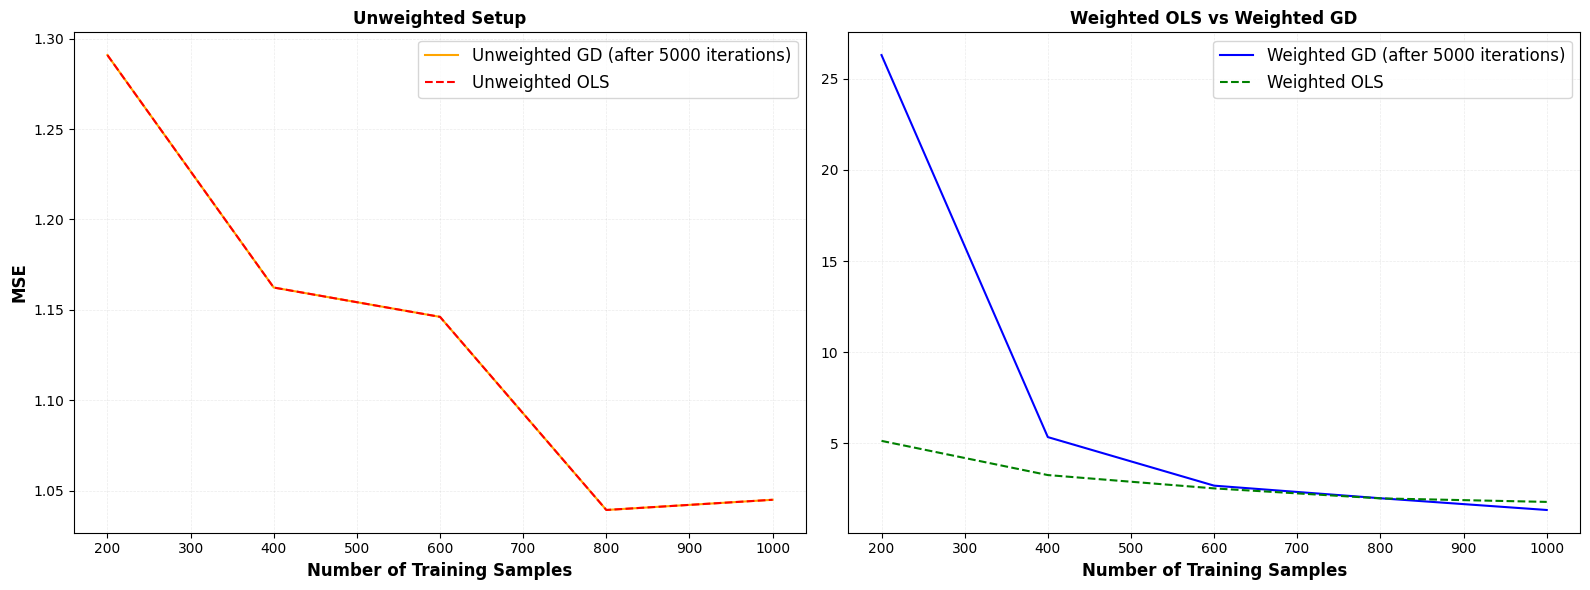
\includegraphics[width=\textwidth]{images/Figure 14.png}
    \captionsetup{format=hang, singlelinecheck=false}
    \caption{Effect of sample size on performance of OLS and gradient descent with step size, $\gamma=0.1$ after $\text{T} = 5000$ iterations in both weighted and unweighted setup.}
    \label{fig:14}
\end{figure}

Our observation from Figure \ref{fig:14} solidifies our learning so far that sample size plays a crucial role in importance weighting. For same number of iterations, the performance of importance weighted gradient descent and convergence with importance weighted OLS depends on the sample size. In our current setup, with $\sim 600$ samples the weighted gradient descent could converge to weighted OLS performance and with even higher sample size ($> 900$), the weighted gradient descent could even beat the performance of weighted OLS.\\

We should also note that in the unweighted setup as well, the performance of gradient descent depends on the sample size. This can be observed in Figure \ref{fig:15}. This is same as the previous figure, but the results are plotted after $\text{T} = 400$ iterations.

\begin{figure}[h!]
    \centering
    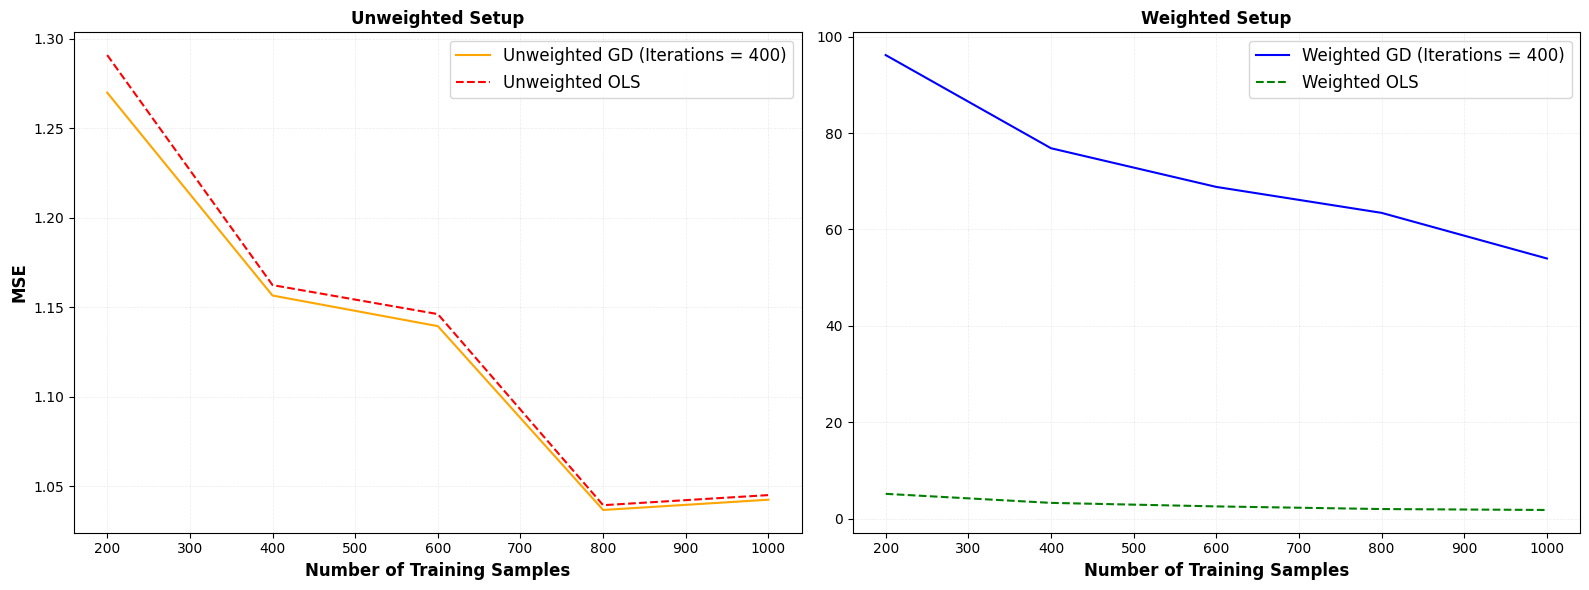
\includegraphics[width=\textwidth]{images/Figure 15.png}
    \captionsetup{format=hang, singlelinecheck=false}
    \caption{Effect of sample size on performance of OLS and gradient descent with step size, $\gamma=0.1$ after $\text{T} = 400$ iterations in both weighted and unweighted setup.}
    \label{fig:15}
\end{figure}

We can observe that in unweighted setup, even with a relatively low iteration of $\text{T} = 400$, a fairly lower sample size is enough for the performance of gradient descent to converge with that of OLS estimator. With higher iterations, even lower sample size can be enough for the convergence. 

\subsection{Self-attention Mechanism}

We recall from section \ref{self-attention} that for an empirical loss

\begin{equation}
    \hat{\mathcal{R}}(\theta, \omega) := \frac{1}{n} \sum_{i=1}^n m(\omega^{(i)})\ell (y_i, \langle \theta, x_i \rangle)
    \label{eqn:21}
\end{equation}

where $\omega = (\omega^{(1)}, \ldots, \omega^{(n)})$ is the importance weights and $m: \mathbb{R} \to \mathbb{R}$ is a masking function, the \textcolor{blue}{\emph{gradient descent-ascent algorithm}} with initial regression parameter, $\theta_0 = 0$ and initial weights, $\omega^{(i)}_0$ for all $i = 1, \ldots, n$ is given by:

\begin{equation}
    \begin{aligned}
        \theta_{t+1} &= \theta_t - \gamma_t \nabla_{\theta} \hat{\mathcal{R}}(\theta_t, \omega_t)\\
        \omega_{t+1} &= \omega_t - \eta_t \nabla_{\omega} \hat{\mathcal{R}}(\theta_t, \omega_t)
    \end{aligned}
    \label{eqn:6.12}
\end{equation}

where $\gamma_t$ and $\eta_t$ are the learning rates.\\

We compute the gradients of the above empirical risk with respect to $\omega$ and $\theta$ by:\\

\begin{equation}
    \begin{aligned}
        \nabla_{\theta}\hat{\mathcal{R}}(\theta, \omega) &= \frac{2}{n}\mathbf{X}^\top\mathbf{M}(\mathbf{X}\theta - \mathbf{Y})\\
        \nabla_{\omega}\hat{\mathcal{R}}(\theta, \omega) &= \frac{1}{n} \frac{dM(\omega)}{d\omega} (\mathbf{X}\theta - \mathbf{Y}) \odot (\mathbf{X}\theta - \mathbf{Y})
    \end{aligned}
    \label{eqn:6.13}
\end{equation}\\

For our experimental purpose, we have kept the step size, $\gamma = 0.1$ and iteration count, $\text{T} = 7500$ for the gradient descent-ascent algorithm. The experiment was carried out at a fixed mean shift, $\mu = 1.0$.\\

Figure \ref{fig:16} shows the effect of masking function is regularizing mean shift. The comparison involves unweighted gradient descent (GD) and weighted GD with Self-Attention-based Masking, using different masking strategies. As we recall from the definition \ref{masking} of masking function, using $q=0$ in the unbounded masking function $m_q(t) = t^q$ gives us unweighted variant, as $q=0$ ignores the effect of weighting.\\

\begin{figure}[h!]
    \centering
    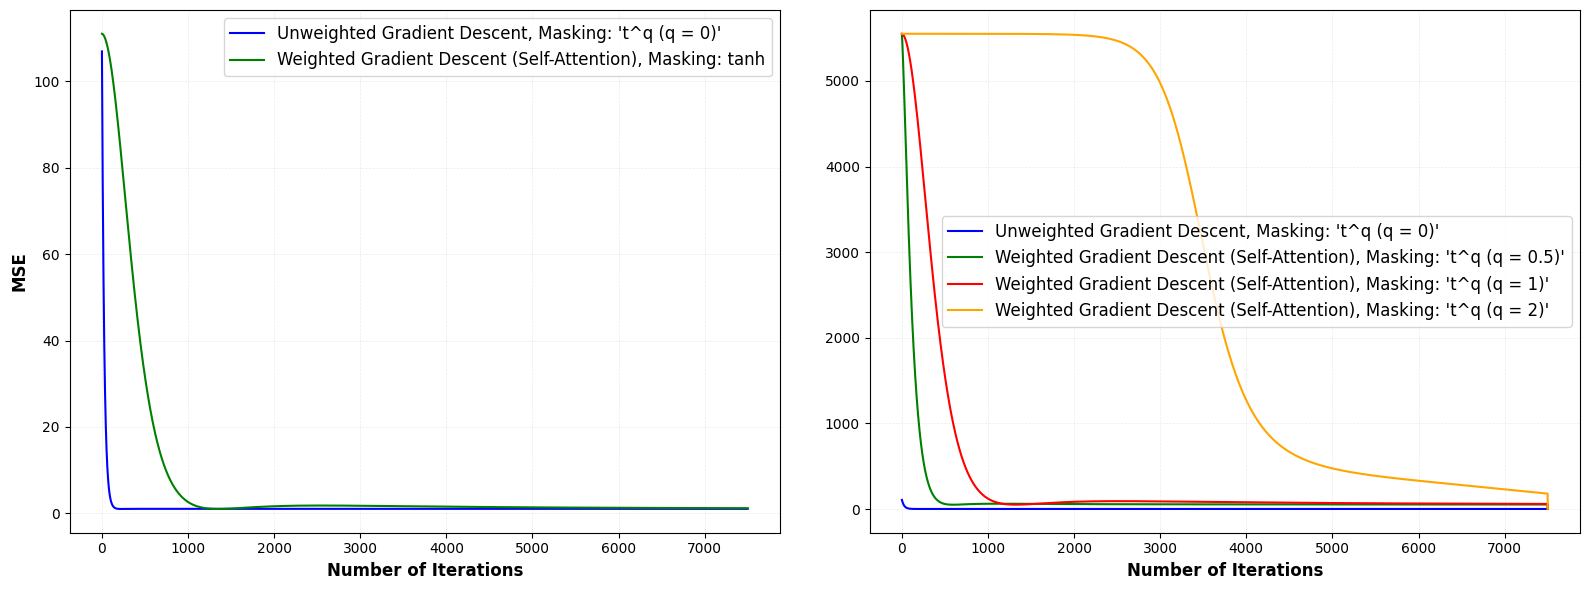
\includegraphics[width=\textwidth]{images/Figure 16.png}
    \captionsetup{format=hang, singlelinecheck=false}
    \caption{Regularizing mean shift by importance weighting using self-attention mechanism. The gradient descent-ascent algorithm was carried out at step size, $\gamma = 0.1$ and for $7500$ iterations. Left: uses $m(t) = tanh(t)$ masking function (bounded). Right: uses $m_q(t) = t^q$ masking function (unbounded) for $q \in [0.5, 1, 2]$.}
    \label{fig:16}
\end{figure}

The left subplot in Figure \ref{fig:16} uses a bounded masking function $m(t) = tanh(t)$. Both unweighted and weighted gradient descent methods exhibit a sharp initial drop in MSE, indicating rapid convergence. After a certain number of iterations ($\sim 1000$), both methods stabilize, reaching nearly the same final MSE. Also, the weighted GD initially decreases slower compared to unweighted GD but eventually reaches similar performance.\\

The right subplot in Figure \ref{fig:16} uses an unbounded masking function $m_q(t) = t^q$ and plots for different values of $q \in [0.5, 1, 2]$. We can observe that for smaller values of $q (=0.5)$, weighted gradient descent converges comparatively faster. However, for larger values of $q$ ($q = 2$), the initial MSE is extremely high, and convergence is much slower, possibly due to overemphasis on certain data points, leading to instability before gradually decreasing. This suggests that \emph{larger $q$ values in the self-attention weighting mechanism can lead to unstable learning process resulting in poor initial performance and slow adaptation}. This behavior aligns with our theoretical expectation from choosing high $q$ value in unbounded masking function $m_q(t) = t^q$, which we discussed in section \ref{choice-masking-q} (Choice of Masking Function).\\

Overall, we also observe from Figure \ref{fig:16} that the initial MSE for bounded masking function $m(t) = tanh(t)$ is much lower than the unbounded masking function $m_q(t) = t^q$. It can also be noted that the unbounded masking function with $q=1$ takes almost same number of iterations to converge to the unweighted gradient descent MSE as the bounded masking function.\\

We also want to see how sample size plays a role in the choice of masking function during the importance weighting with self-attention mechanism. 

\begin{figure}[h!]
    \centering
    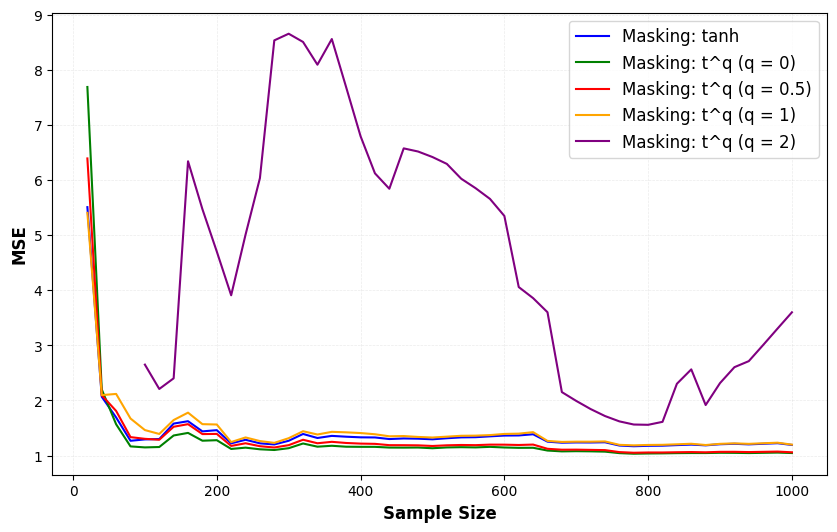
\includegraphics[width=0.8\textwidth]{images/Figure 17.png}
    \captionsetup{format=hang, singlelinecheck=false}
    \caption{Effect of sample size on mean shift regularization with weighted gradient descent (step size, $\gamma = 0.1$ and number of iterations $=7500$) using self-attention mechanism. Here, we use different masking functions, both unbounded and bounded.}
    \label{fig:17}
\end{figure}

In Figure \ref{fig:17}, we observe that with same sample size ($n = 1000$), unbounded masking function with low value of $q$ ($q=0.5$) gives the best result for low sample sizes. We note here that the green line corresponding to $q=0$ is the unweighted gradient descent here. For higher sample sizes ($>800$), the performance of most masking functions are almost similar with very less difference. We can easily observe that the only exception is the unbounded masking function $m_q(t) = t^q$ with highest value of $q$ ($q=2$), because high value of $q$ leads to unstable learning process. This aligns with our observation from Figure \ref{fig:16} and theoretical expectations discussed in section \ref{choice-masking-q} (Choice of Masking Function). 